\section*{Process description}

Nitroma's process for the nitration of toluene and subsequent reduction and hydrogenation of nitrotoluenes is unique in both its continuous operating mode and the capability of producing three different substituted aromatic amines.  \Cref{fig:BFD-ES} is a simplified process flow diagram of the process.

Firstly, toluene is nitrated with \SI{70}{\percent} aqueous nitric acid in a shell-and-tube heat exchanger reactor packed with H-Mordenite solid catalyst. Solid acid catalysts were preferred over the traditional mixed-acid synthesis due to environmental, safety and performance advantages. Zeolites alleviate the need for costly and energy intensive regeneration of corrosive sulphuric acid and prevent the emission of toxic greenhouse gases such as nitrogen oxides. Heterogeneous catalysis is also attractive from an economical point of view since it favours the more economically desirable \para-nitrotoluene (PNT) isomer. 

\begin{wrapfigure}{r}{0pt}
    \centering
    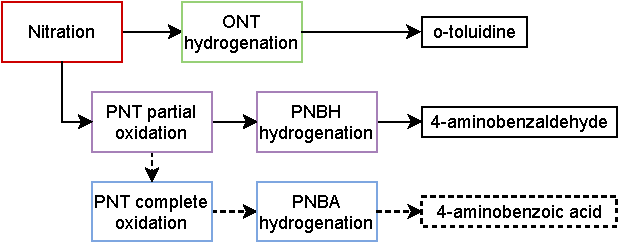
\includegraphics[width=0.4\linewidth]{chapters/0-executive-summary/figures/BFD_nitroma-simplifed.pdf}
    \caption{Simplified synthesis route for Nitroma's process}
    \label{fig:BFD-ES}
\end{wrapfigure}
The nitration reactor effluent is fed to a decanter to separate the aqueous nitric acid from the organic phase. Following water evaporation in a distillation column, nitric acid is recycled back into the nitration reactor at a \SI{99.8}{mol\percent} purity. Meanwhile, the organic phase is sent to a distillation column to recycle unreacted toluene to the nitration reactor. The nitrotoluenes are sent to a second distillation column to separate the more volatile \ortho-nitrotoluene (ONT) from \meta-nitrotoluene (MNT) and PNT. The large difference in the PNT and MNT melting points is exploited in a mixed-suspension mixed-product removal crystalliser, followed by a hydraulic wash column.

Liquid ONT is mixed with methanol and hydrogenated under pressure over Pd/C catalyst to \ortho-toluidine (o-TOL) in a downflow co-current trickle bed reactor. A trickle bed reactor was chosen due to the ease of operation at high pressure and relatively slow catalyst deactivation, which is imperative for an expensive catalyst such as Pd/C. o-TOL is then purified to achieved a purity of \SI{99.4}{mol\percent}. The excess hydrogen gas leaves the reactor via an outlet port, and the effluent enters a distillation column to separate methanol and water from the less volatile organic compounds. Methanol is further distilled to be recycled to the reactor. 

Meanwhile, gaseous PNT is fed into an air-oxidation reactor packed with cobalt phthalocyanine catalyst to be partially oxidised to 4-nitrobenzaldehyde (4-NBH). Nitroma's two production campaigns allow the reactor effluent to either be sent to a second oxidation reactor where 4-NBH and unreacted PNT will be completely oxidised to 4-nitrobenzoic acid (4-NBA) in the BA scenario; or directly to a liquid-phase hydrogenation reactor in the BH scenario. Ultimately, 4-NBH and 4-NBA are both reduced to respectively 4-aminobenzaldehyde (4-ABH) and 4-aminobenzoic acid (4-ABA) with formic acid diluted in a methanol solvent over Pt/C catalyst. 4-ABH is purified via a sequence of distillation packed columns whereas 4-ABA is recovered as a solid following  crystallisation in a continuous falling-film melt crystalliser.








 

